%-------------------------------------------------------------------------------
%	Packages and other Document configurations
%-------------------------------------------------------------------------------
\documentclass[a4paper,11pt]{article}\usepackage[]{graphicx}\usepackage[]{xcolor}
% maxwidth is the original width if it is less than linewidth
% otherwise use linewidth (to make sure the graphics do not exceed the margin)
\makeatletter
\def\maxwidth{ %
  \ifdim\Gin@nat@width>\linewidth
    \linewidth
  \else
    \Gin@nat@width
  \fi
}
\makeatother

\definecolor{fgcolor}{rgb}{0.345, 0.345, 0.345}
\newcommand{\hlnum}[1]{\textcolor[rgb]{0.686,0.059,0.569}{#1}}%
\newcommand{\hlstr}[1]{\textcolor[rgb]{0.192,0.494,0.8}{#1}}%
\newcommand{\hlcom}[1]{\textcolor[rgb]{0.678,0.584,0.686}{\textit{#1}}}%
\newcommand{\hlopt}[1]{\textcolor[rgb]{0,0,0}{#1}}%
\newcommand{\hlstd}[1]{\textcolor[rgb]{0.345,0.345,0.345}{#1}}%
\newcommand{\hlkwa}[1]{\textcolor[rgb]{0.161,0.373,0.58}{\textbf{#1}}}%
\newcommand{\hlkwb}[1]{\textcolor[rgb]{0.69,0.353,0.396}{#1}}%
\newcommand{\hlkwc}[1]{\textcolor[rgb]{0.333,0.667,0.333}{#1}}%
\newcommand{\hlkwd}[1]{\textcolor[rgb]{0.737,0.353,0.396}{\textbf{#1}}}%
\let\hlipl\hlkwb

\usepackage{framed}
\makeatletter
\newenvironment{kframe}{%
 \def\at@end@of@kframe{}%
 \ifinner\ifhmode%
  \def\at@end@of@kframe{\end{minipage}}%
  \begin{minipage}{\columnwidth}%
 \fi\fi%
 \def\FrameCommand##1{\hskip\@totalleftmargin \hskip-\fboxsep
 \colorbox{shadecolor}{##1}\hskip-\fboxsep
     % There is no \\@totalrightmargin, so:
     \hskip-\linewidth \hskip-\@totalleftmargin \hskip\columnwidth}%
 \MakeFramed {\advance\hsize-\width
   \@totalleftmargin\z@ \linewidth\hsize
   \@setminipage}}%
 {\par\unskip\endMakeFramed%
 \at@end@of@kframe}
\makeatother

\definecolor{shadecolor}{rgb}{.97, .97, .97}
\definecolor{messagecolor}{rgb}{0, 0, 0}
\definecolor{warningcolor}{rgb}{1, 0, 1}
\definecolor{errorcolor}{rgb}{1, 0, 0}
\newenvironment{knitrout}{}{} % an empty environment to be redefined in TeX

\usepackage{alltt}
% Package declaration
%-------------------------------------------------------------------------------
% Specify input encoding
\usepackage[utf8]{inputenc}
% For A4 paper set all margins to 3cm
\usepackage[paper=a4paper,left=1.5cm,top=2cm,right=1.5cm,bottom=2cm]{geometry}%
% Set linespace, usage \doublespacing \singlespacing \onehalfspacing
\usepackage{setspace}%
% Set palatino font with small caps as default
\usepackage[sc]{mathpazo}%
% Rotation tools, including rotated full-page floats.
\usepackage{rotating}%
% Create subfigures
\usepackage{subfigure}%
% Extensive support for hypertext in LaTeX
\usepackage{hyperref}%
% For adding bookmarks to the document
\usepackage{bookmark}%
% For adding time to the document
\usepackage{datetime}
% For alignment of captions
\usepackage{caption}
% For multiple columns.
\usepackage{multicol}

% Start Article header
%-------------------------------------------------------------------------------
% Title
\title{AMMI report for grain.yield}%
% Authors
\author{\vspace{-5ex}}
%-------------------------------------------------------------------------------
% Dates
\date{\vspace{-5ex}}
%-------------------------------------------------------------------------------
% End article header

% For left aligning captions
\captionsetup{justification=raggedright,singlelinecheck=false}

% Start Document
%-------------------------------------------------------------------------------
\IfFileExists{upquote.sty}{\usepackage{upquote}}{}
\begin{document}

% Article title and date.
\maketitle
% Start single line spacing
\singlespacing

%-------------------------------------------------------------------------------
\section{General information}
%-------------------------------------------------------------------------------

% latex table generated in R 4.3.0 by xtable 1.8-4 package
% Fri Nov 24 08:09:25 2023
\begin{table}[ht]
\begin{flushleft}
\begin{tabular}{ll}
  Analysis done on & 23-11-24 07:47:00 \\ 
  statgenGxE version & 1.0.5 \\ 
  \end{tabular}
\label{general}
\end{flushleft}
\end{table}


%-------------------------------------------------------------------------------
\section{Anova tables}
%-------------------------------------------------------------------------------

% latex table generated in R 4.3.0 by xtable 1.8-4 package
% Fri Nov 24 08:09:25 2023
\begin{table}[ht]
\begin{flushleft}
\label{anova}
\begin{tabular}{lrrrrrl}
  \hline
 & Df & Sum Sq & Mean Sq & F value & Pr($>$F) &  \\ 
  \hline
Trial & 9 & 23677 & 2631 & 2970.19 & 0.00E+00 & *** \\ 
  Genotype & 245 & 2321 & 9 & 10.69 & 2.55E-237 & *** \\ 
  Interactions & 2205 & 1953 & 1 &  &  &  \\ 
  PC1 & 253 & 622 & 2 & 4.18 & 0.00E+00 & *** \\ 
  PC2 & 251 & 330 & 1 & 2.24 & 0.00E+00 & *** \\ 
  Residuals & 1701 & 1000 & 1 &  &  &  \\ 
   \hline  \multicolumn{6}{c}{Significance codes: 0 '***' 0.001 '**' 0.01 '*' 0.05 '.' 0.1 ' ' 1 } \\ \hline
\end{tabular}
\end{flushleft}
\end{table}

\clearpage
%-------------------------------------------------------------------------------
\section{PCA Summaries}
%-------------------------------------------------------------------------------

% latex table generated in R 4.3.0 by xtable 1.8-4 package
% Fri Nov 24 08:09:25 2023
\begin{table}[ht]
\begin{flushleft}
\scalebox{1}{
\begin{tabular}{lcc}
  \hline
 & PC1 & PC2 \\ 
  \hline
Standard deviation & 1.59 & 1.16 \\ 
  Proportion of Variance & 0.32 & 0.17 \\ 
  Cumulative Proportion & 0.32 & 0.49 \\ 
   \hline
\end{tabular}
}
\label{importance}
\end{flushleft}
\end{table}


\begin{knitrout}
\definecolor{shadecolor}{rgb}{1, 1, 1}\color{fgcolor}\begin{kframe}
\end{kframe}

\includegraphics[width=\maxwidth]{./figures/112423080925-impPlot-1} \hfill{}


\end{knitrout}
\newpage

%-------------------------------------------------------------------------------
\section{Biplots}
%-------------------------------------------------------------------------------
\begin{knitrout}
\definecolor{shadecolor}{rgb}{1, 1, 1}\color{fgcolor}\begin{kframe}
\end{kframe}
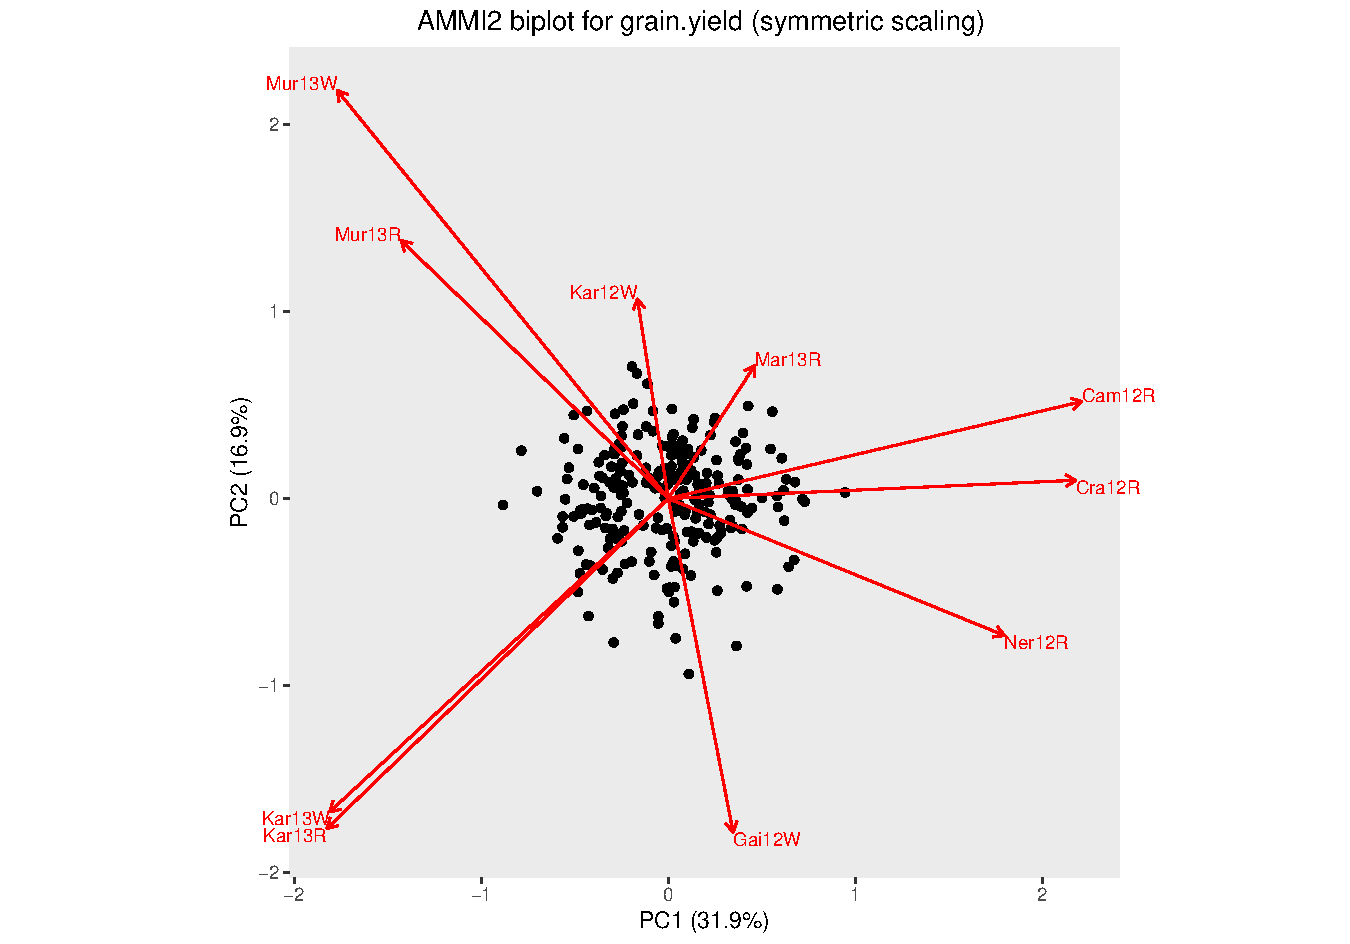
\includegraphics[width=0.9\maxwidth]{./figures/112423080925-biplot-1} 
\end{knitrout}

%-------------------------------------------------------------------------------
% End Document
\end{document}
